\section{Aufbau und Durchführung}
\label{sec:Durchführung}
Bei dem Versuch wird eine Messapparatur wie in \autoref{fig:Abb_8} benutzt mit einer Verbindung zu einem elektronischen Zählwerk.
In dem Versuch ist eine Strahlungsquelle in einer Halterung befestigt, welche von einer Abschirmung umgeben ist, wodurch die Strahlung nicht zur Seite entweichen kann.
In einem gewissen Abstand befindet sich ein Plattenhalter, in den Platten unterschiedlicher Dicke einspannen werden können.
Dahinter ist ein Geiger-Müller-Zählrohr, mit dem die Intensität der Strahlung gemessen wird. 
Der ganze Aufbau ist auch nochmal mit einer Abschirmung umgeben, damit die Strahlung nach außen hin abgefangen wird und die Apparatur
vor äußeren Einflüssen geschützt wird.
\begin{figure}[H]
    \centering
    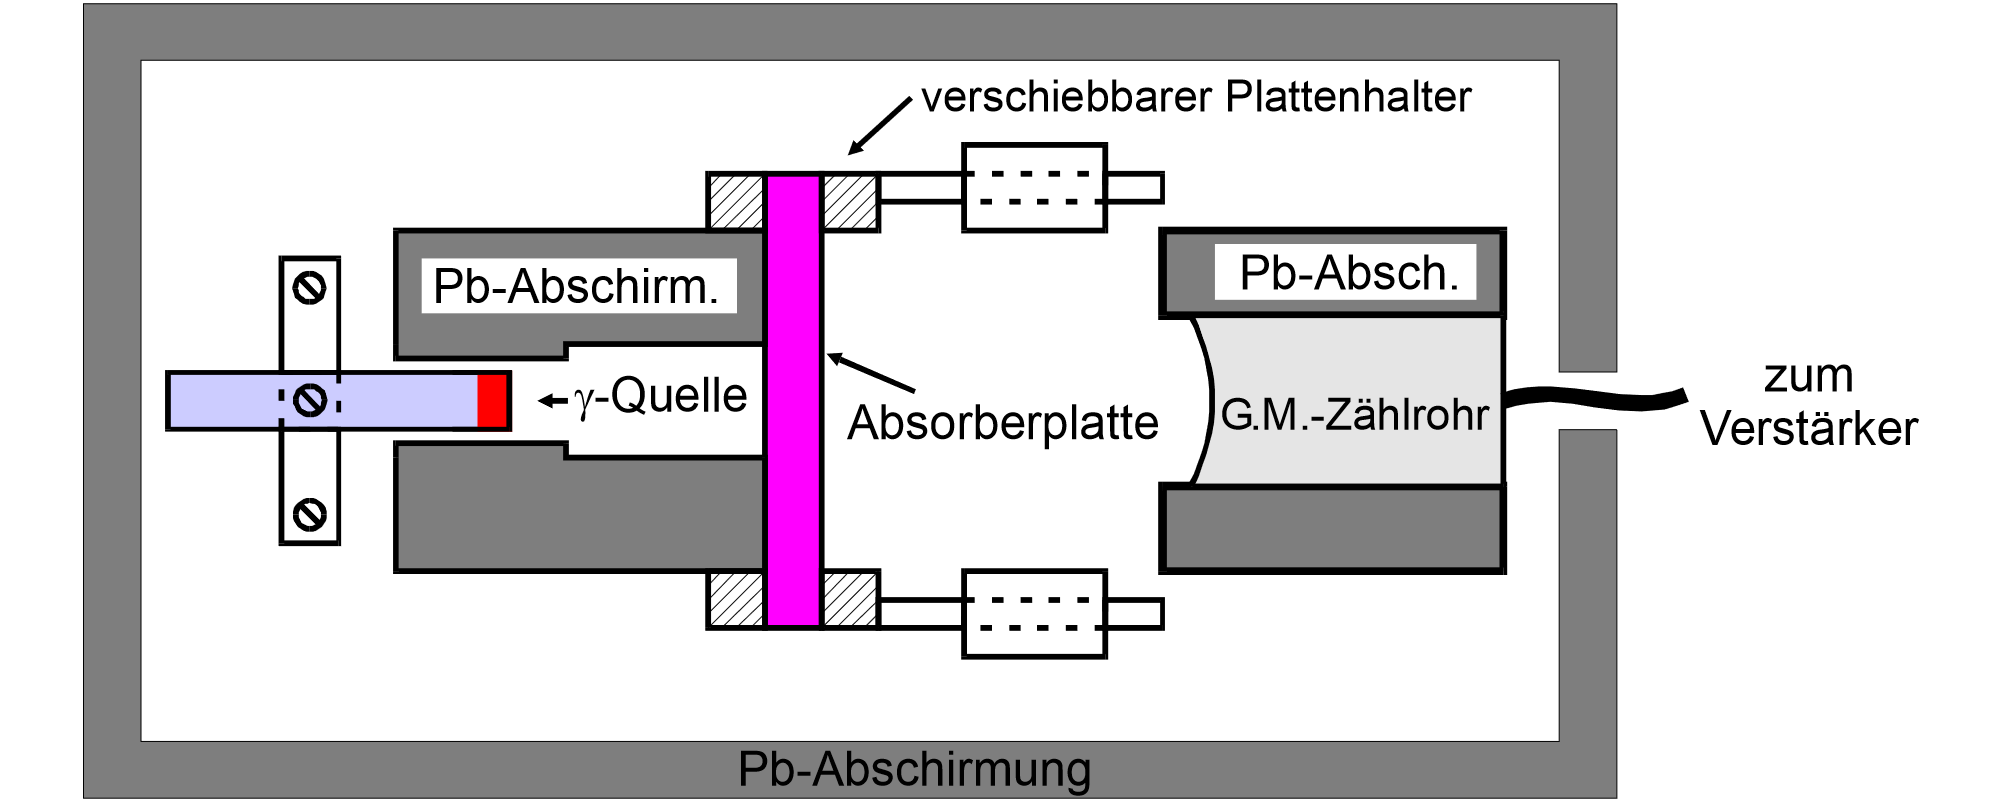
\includegraphics[width=0.5\textwidth]{build/Abb_8.png}
    \caption {Schematische Darstellung der Messapparatur\cite[243]{V704}.}
    \label{fig:Abb_8}
\end{figure}
Zur Beginn der Messungen wird der Nulleffekt gemessen. 
Es wird über einen hinreichend langen Zeitraum (900 Sekunden) die Zählrate ohne jeglichen Einfluss eines extra eingebauten Strahlers gemessen.\\
Anschließend wird eine Quelle eingebaut und bei unterschiedlichen Dicken der Absorberplatte die Zählrate über einen entsprechend langen Zeitraum (je dicker die
Platte, desto länger der Zeitraum) gemessen.
Die Dicke, die Zählrate und die Zeit wird ein einer Tabelle aufgetragen.
Diese Messung wird für die $\gamma$- und $\beta$-Strahlung analog durchgeführt.
